\chapter{Обзор литературы}
\label{chap:lr}
\chaptermark{Обзор литературы}

\section{Традиционная архитектура компиляторов}
\label{sec:review_1}

С середины $20^{го}$ века, благодаря усилиям работников индустрии разработки ПО, а также научным исследованиям, был сделан большой прорыв в разработке компиляторов с акцентом на классическую задачу компиляции: 
создание быстрого и эффективного объектного кода для выполнения на виртуальной
машине или микропроцессоре.


Однако другие возможности компиляторов, такие как инструменты анализа кода, 
способные предоставлять исчерпывающую информацию о семантике программного кода,
остаются необычным и редким качеством современных компиляторов для популярных языков программирования.

Наиболее наглядно эту проблему можно наблюдать в инструментах разработки для Java:

Код Java обычно компилируется с использованием компилятора Sun Java. "Будучи
монолитной программой, построенной по принципу ``черного ящика" \cite{Zouev2005}, 
Sun Java способен лишь принять исходный код и сгенерировать из него байткод для виртуальной машины Java.


В то же время современная среда разработки включает в себя набор инструментов,
упрощающих работу программиста, и требует предварительного анализа синтаксиса и семантики кода, 
что не представляется возможным без построения Семантического Представления\cite{Zouev2005}. 
Построение такого представления требует реализовать основную функциональность компилятора заново.


Глядя в прошлое, легко понять причины этой проблемы: 
традиционно программы рассматривались как простые текстовые объекты
преобразующиеся в исполняемый код. Согласно этому предположению, компиляторы
были спроектированы очень логично: они не не хранили никакой информации о семантике исходного кода, 
помимов некоторых низкоуровневых внутренних промежуточных представлений.


Промежуточные представления этих компиляторов имели очень ограниченный набор вариантов использования \cite{Zouev2005, Zouev2010}, более того, они
хорошо подходили для единственной задачи: генерации объектного кода для набора поддерживаемых микропроцессоров. 
Также внутреннее представление компилятора нестабильно и имеет тенденцию очень активно меняться
во время разработки компилятора \cite{FreeSoftwareFoundation2016}. Следовательно, внутреннее представление компилятора не может 
быть использовано для построения средств анализа кода.

Ситуация с инструментарием C++ еще более удручающая: синтаксис языка
и семантика намного сложнее, чем у Java, поэтому создание альтернативного
компилятора --- весьма непростая задача даже для большого бизнеса.

В результате мы можем наблюдаеть заметный недостаток инструментов для C++\cite{Zouev2010}, а существующие
довольно сложны в реализации: среда разработки JetBrains CLion имеет собственный парсер
и семантический анализатор для реализации функций автодополнения, рефакторинга и статического анализа,
основанные на собственном семантическом представлении языка C++. 
Будучи сложным программным продуктом, парсер CLion, имеет собственные недостатки и 
отстает от развития языка на несколько месяцев после выхода нового стандарта.


Microsoft Visual Studio "страдает" от той же проблемы: VC++ генерирует промежуточное представление, пригодное
только для генерации кода: внутреннее представление сильно фрагментировано и очень низкоуровнево.
Набор инструментов C\&C++ IntelliSense в интегрированной среде разработки Microsoft Visual Studio 
полностью отделен от компилятора VC++ и реализует свой собственный парсер и семантический анализатор.

\section{Современные компиляторы и СП}
\label{sec:review_2}

Несмотря на то, что традиционные компиляторы сегодня широко используются, их
возможности по интеграции в среды разработки давно исчерпаны и всё больше новых языков сейчас
нацелены на реализацию семантического представления как стабильного промежуточного представления,
которое можно использовать во внешних инструментах семантического анализа.

Согласно \cite{Zouev2005, Zouev2010}, в отличие от промежуточного представления традиционного компилятора, 
семантическое представление содержит полный спектр ``знаний'' о программе, и включает в себя все аспекты, которые подразумеваются 
в исходном коде. Это дает возможность строить мощные инструменты, основанные на семантическом анализе.

\begin{itemize}
\item генерация кода
\item распределенная (или рекурсивная) проверка синтаксиса
\item человекопонятная визуализация
\item статический анализ
\item интерпретация программы
\item Семантический поиск: очень мощный метод запроса семантических объектов кода (пример: "найти все классы, производные от класса C, которые не переопределяют виртуальную функцию f”)
\end{itemize}

Существует три основных пути описания семантического представления и предоставления доступа к нему извне:
предоставление доступа к программному интерфейсу, который реализует доступ и модицикацию элементов семантического представления\cite{Cannon, FreeSoftwareFoundation2016}
отображение семантического представления на реляционную базу данных\cite{Linton1983},
и предоставление доступа к семантическому представлению в виде текста, используя открытый формат структурирования данных\cite{TheRustTeam2016}.

Цитируя \cite{Zouev2005}, ``API является универсальным способом реализации любой требуемой функциональности, 
но в условиях меняющихся требований, невозможно предугадать спектр потребностей клиентов''.
Открытый формат семантического представления, в свою очередь может стать решением потенциальной проблемы: ``Обычно доступ к открытому формату можно получить несколькими способами:
от простых API до высокоуровневых специалилированных программных продуктов. Кроме того, возможна реализация собственных инстерфейсов обработки семантического представления, выраженного в открытом формате''

%WTF is this???
And an open SP format can be a solution to potential problems: ``open formats

Конкретным форматом может являться как нечто собственной разработки, так и унифицированное стандартное решение, 
такое как XML\cite{Germon} или JSON\cite{ECMA-4042013}.

\newpage
\section{LSP and distributed approach to building development environment}
\label{sec:review_3}
Учитывая вышеизложенное, в настоящее время мы имеем прочную основу для обеспечения хорошего инструментария, 
основанного на семантическом анализе: методов представления семантического представления исходного кода программного обеспечения 
и его оценки в соответствии с потребностями клиентов.

Современные IDE применяют эти методы для предоставления достойного сервиса, но все же существует проблема: 
эти программные продукты используют свои собственные реализации компиляторов, обычно несвободные и не связанные с командой разработчиков исходного языка. 
Это подразумевает набор проблем, отмеченных в \ref{sec: review_1}.

Наличие хорошего современного компилятора, способного генерировать SR, делает вещи немного менее сложными, 
но все же не решает проблему времени и стоимости реализации IDE для конкретного языка.

Очевидно, что эти проблемы не являются уникальными для класса продуктов IDE, но для любой большой монолитной архитектуры, 
и решение может быть довольно простым: если мы можем снизить связывание системы и представить среду разработки в виде набора инструментов 
вместо одного интегрированного решения, мы можем распределить реализацию IDE, чтобы иметь набор несвязанных модулей:
\begin{itemize}
    \item Редактор кода
    \item Комилятор, предоставляющий семантическое представление
    \item Клиенты семантического представления (см. \ref{sec:review_1})
    \item Протокол, объединяющий клиенты и компилятор
\end{itemize}
\newpage

\begin{figure}[H]
    \centering
    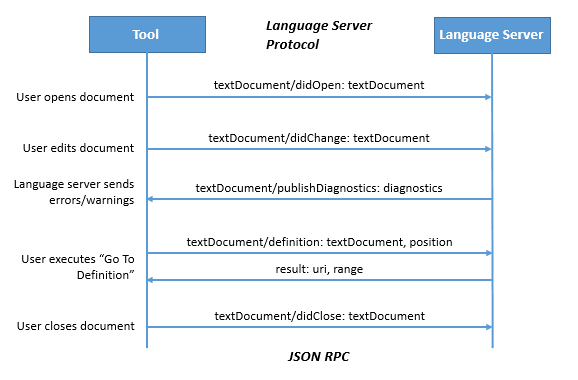
\includegraphics[width=0.85\textwidth]{figs/lsp.png}
    \caption{Протокол, объединяющий клиенты и компилятор}
\end{figure}

Описанный протокол уже существует -- Протокол Языкового Сервера (LSP --- Language Server Protocol) удовлетворяет потребность в подключении сторонних инструментов, давая возможность
реализовать функциональность полноценной IDE, избегая расходы на содержание и развитие отдельного монолитного программного продукта.

Языковой Сервер и протокол языкового сервера, разработанные корпорацией Microsoft в 2016 году, предлагает представить среду разработки как две слабо связанные стороны:
\begin{itemize}
    \item Языковой Сервер, реализующий анализ семантического представления и основанные на нём утилиты.
    \item Клиенты, в качестве которых выступают редакторы кода и другие инструменты разработчика, использующие протокол языкового сервера для связи с языковым сервером\cite{Sourcegraph}.
\end{itemize}

\section{Заключение}
\label{sec:review_conclusion}
Обычные компиляторы с монолитной архитектурой, которые хороши только при генерации исполняемого кода, 
трудно интегрировать в современную среду разработки, поскольку они не разделяют семантическое представление исходного кода, 
поэтому для разработки хорошей IDE необходимо написать свой собственный исходный код компилятора для семантического представления.

Современный компилятор (который предоставояет промежуточное представление высокого уровня) --- это большой шаг к упрощению разработки утилит разработчика, 
дающий большие преимущества в затратах времени и финансов в сочетании с распределенной архитектурой IDE, разделяющей редактор и набор инструментов для анализа семантики языка 
на две непересекающиеся части и связывая их через стандартизированный протокол.

Такой подход дает разработчикам языка большие возможности для развития инфраструктуры языка,
которые могут предоставить набор инструментов анализа через языковой сервер, 
а также дает возможность способ экспериментировать с новыми и существующими методами семантического анализа.
Например, База Знаний о ПО\cite{Wanghong}, описанная Бертраном Мейером, может быть реализована как модуль языкового сервера,
в качестве альтернативы подходу, выбранному авторами в 1985 году: интеграция инструментов анализа в редактор не представлялась возможной в то время, 
а это именно то, для чего языковой сервер подходит наилучшим образом.

В заключение следует отметить, что языковой сервер может быть рассмотрен как наиболее приемлемое решение для быстрого развертывания богатой инфраструктуры языка,
что особенно важно для новых языков программирования.